% !TEX root=/home/tavant/these/manuscript/src/manuscript.tex

\section{Instability in the \ac{PIC} simulation}
  \label{sec-PIC-ECDI}
  As briefly mentioned in \cref{ch-1}, the $E \times B$ configuration of the \ac{HET} make azimuthal instabilities to rise.
  This aspect has been neglected in \cref{ch-2,ch-3}, expect when talking about the axial electron transport.
  While these instabilities are the subject of numerous studied, they remain unclear.
  
  Using the results of the \ac{PIC} simulation, we propose some new insights for the understanding on the instability, hence the electron cross-field transport. 
  \inlinenote{Maybe this part in the chapter abstract...?}
  
  We present in this section the results obtained for one case.
  However, we observe the same results when varying the  different physical parameters.
  The parameters of the simulations are presented in \cref{tab-evdfpicparams}.
  The radial boundary condition include a dielectric layer, of width $L_{diel}$.
  No electron emission is modeled, and the convection is modeled with the new model (see \cref{sec-noiselessresults}).

  \begin{table}[hbtp]
  \ra{1.3}
    \centering
    \caption{Parameters of the \ac{PIC} simulations}
    \label{tab-evdfpicparams}
    \begin{tabular}{@{}l l l @{}} \toprule
    Parameter    &   Value   &  Unit  \\ \midrule
    $L_r\times L_{\theta}\times L_z$   & $1\times 0.26\times 0.5$ & cm \\
    $n_e = n_i$  & $\sn{3}{17}$ & \per\meter\cubed \\
    $B_r$  & 0.02 & T \\
    $E_z$  & \sn{2}{4} & \volt\per\meter \\
    $L_{diel}$ & 3 & \milli\meter  \\
    \bottomrule
    \end{tabular}
  \end{table}

  \subsection{Azimuthal electric field}
  
  \Cref{fig-2DcutEx} shows the temporal evolution of the azimuthal electric field as a function of the azimuthal position, measured at the center of the radial direction.
  We clearly see the instability growth up to the saturation around $T=1\,\micro\second$.
  Then, we see in addition to the fast oscillation a slower modulation of the amplitude. 
  \begin{figure}[hbtp]
    \centering
    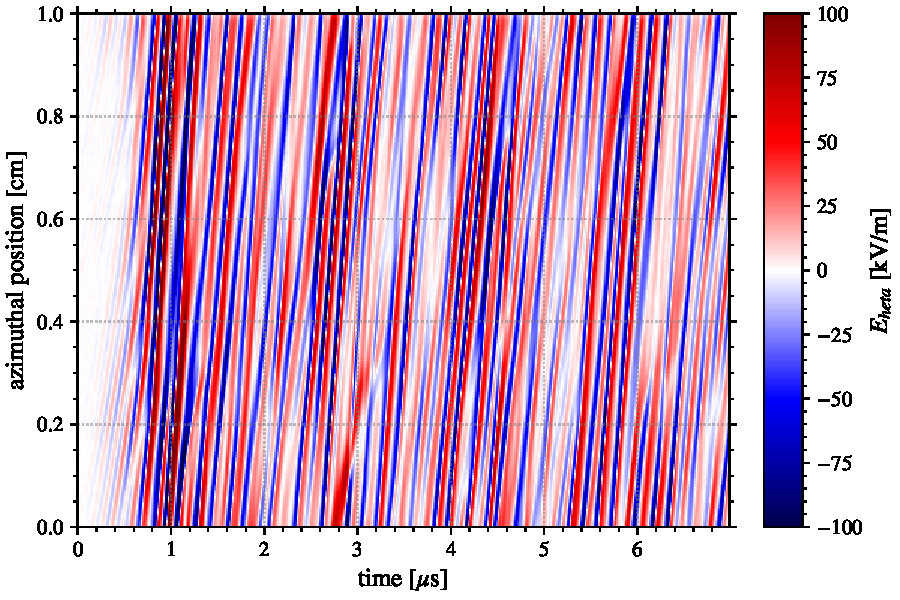
\includegraphics[width=\defaultwidth]{electric_field_cut2D}
    \caption{Temporal evolution of the azimuthal electric field as a function of the azimuthal position.}
    \label{fig-2DcutEx}
  \end{figure}

  \Cref{fig-FFT_ex} shows the frequency spectrum of the azimuthal electric field presented in \cref{fig-2DcutEx} computed via \ac{FFT} in the stationary state ($t > 1.2\,\micro\second$).
  The spectrum have been average in the azimuthal direction, in order to reduce the noise.
  The theoretical frequency $f_{\rm theo} = \frac{\opi}{\pi \sqrt{6} }$ is given. {\bf REF}
  We can see a very good agreement between $f_{\rm theo}$ and the maximum of the frequency spectrum.
  \begin{figure}[hbtp]
    \centering
    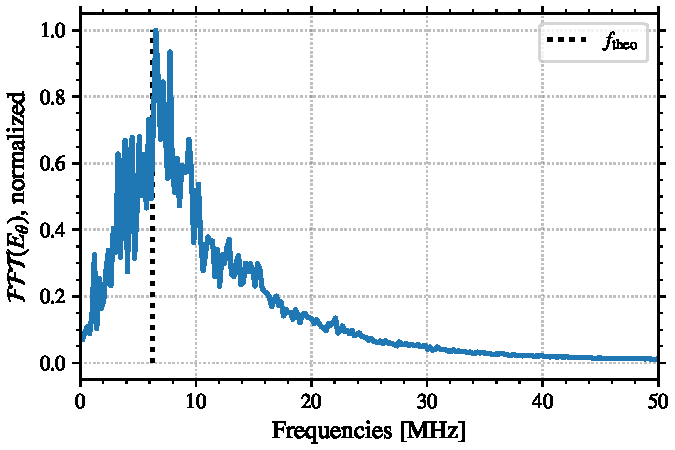
\includegraphics[width=\defaultwidth]{spectrum_frequency}
    \caption{Frequency spectrum of the azimuthal electric field, averaged in the azimuthal direction. The black line is the theoretical frequency.}
    \label{fig-FFT_ex}
  \end{figure}
  
  \subsection{Temporal evolution} \label{subsec-temp}
  We have seen in the previous section that after a growing phase, the instability saturate but oscillates slowly around.
  This section analyse these temporal characteristics.
  
  \Cref{fig-Ezstd_time} shows the temporal evolution of the characteristics of the electrostatic wave.
  As the wave is not monochromatic (i.e. it is the sum of multiple waves), we display both the maximum of the electric field $\max(E_{\theta})$, and its standard deviation $\stdE$.
  In the case of a monochromatic wave, the would have 
  \[ \stdE = \frac{\max(E_{\theta})}{\sqrt{2}}.  \]
  
  \begin{figure}[hbtp]
    \centering
    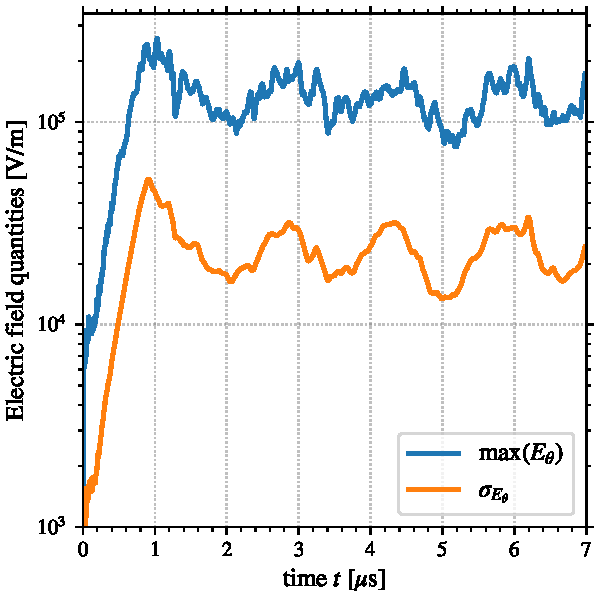
\includegraphics[width=\defaultwidth]{Temporal_E_theta.pdf}
    \caption{Temporal evolution of the maximum and the standard deviation of the azimuthal electric field, in log scale.}
    \label{fig-Ezstd_time}
  \end{figure}
  
  We can see in \cref{fig-Ezstd_time} that during the first microsecond, we observe an exponential growth, corresponding to a constant growth rate.
  A linear fit in log scale give $\gamma_{PIC} \simeq 0.07 \opi$ during the linear phase.
  After $t=1\,\micro\second$, the amplitude of the electric field oscillates around a mean value, with a period of the order of $T_{NL}=1.5 \,\micro\second$.
  Several phenomena are candidate to the modulation observed.
  
  
  \paragraph{Ion transit time\\}
    The ion are injected at the anode, and are accelerated by the uniform axial electric field $E_z$.
    The transit time of the ions in the axial direction $T_t$  is the time needed for the ions to travel $L_z$
    \begin{equation} \label{eq-transittime}
      T_{t} = \sqrt{\frac{2 m_i L_z}{e E_z}} \simeq 0.8 \mu s.
    \end{equation}
    
    The transit time is of the good  order of magnitude, but $T_{NL}$ is twice bigger, still.
    
  \paragraph{Particle trapping and bouncing\\}
    A common raison for wave saturation is the ion trapping. 
    It as been observed in both \ac{1D} \citet{lafleur2016a} and \ac{2D} \citep{croes2017a}.
    
    Hence, the low frequency modulation could be due to particle bouncing \citep{belmont2013}.
    However, the bouncing time scale is 
    \begin{equation} \label{eq-TB}
      T_{B} = 2 \pi \sqrt{\frac{m_i}{e k \max(E_{\theta})} } \simeq 0.5 \,\micro\second,
    \end{equation}
    which is 3 times smaller than $T_{NL}$.
    Even though in \citet{belmont2013}, the authors say that, when the amplitude of the electric field is large (as it is the case here), the bouncing time scale increases due to non-linear phenomenon (the particle trajectory is not harmonic any more), we cannot conclude here that this is the origin of the low frequency modulation.

  
  \paragraph{Ion trapping oscillation\\}
    The wave saturating due to ion trapping have an amplitude of \citep{boeuf2018}
     \begin{equation} \label{eq-iontropempl}
       \stdE \leq \frac{\Te}{12 \lde}.
     \end{equation}
    
    Defining the wave energy  density
    \begin{equation} \label{eq-waveE}
      \epsilon_{\rm wave} = \frac{\epsilon_0}{2} \stdE^2
    \end{equation}
    and the electron thermal energy density
    \begin{equation} \label{eq-thE}
      \epsilon_{\rm th} = \frac{3}{2} e n_e \Te
    \end{equation}
    
    We find the criteria for the ion trapping
    \begin{equation} \label{eq-criteriaIT}
      432 \epsilon_{\rm wave} \leq \epsilon_{\rm th}.
    \end{equation}
    
    \Cref{fig-tempITcrit} shows the temporal evolution of the electron thermal energy $\epsilon_{\rm th}$ and the wave energy density $\epsilon_{\rm wave}$, scaled by the factor 432.
    We can see that $\epsilon_{\rm th}$ is relatively constant.
    However, $\epsilon_{\rm wave}$  oscillates significantly, and passes above and below $\epsilon_{\rm th}$.
    
    \begin{figure}[hbtp]
      \centering
      % 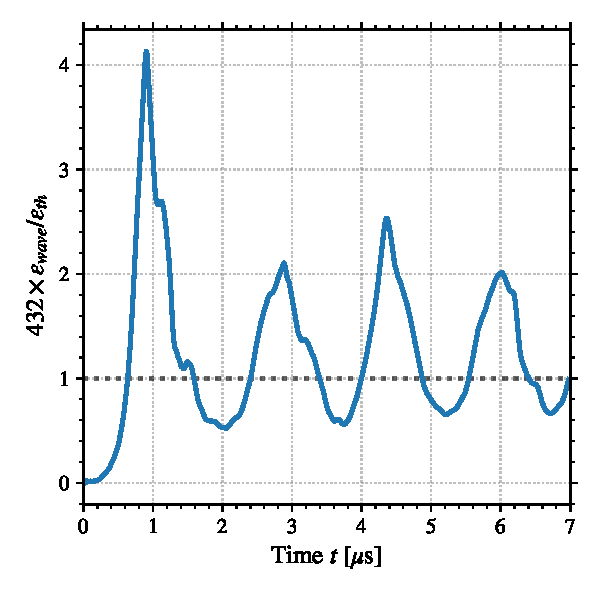
\includegraphics[width=\defaultwidth]{Ion_Trapping_criter}
      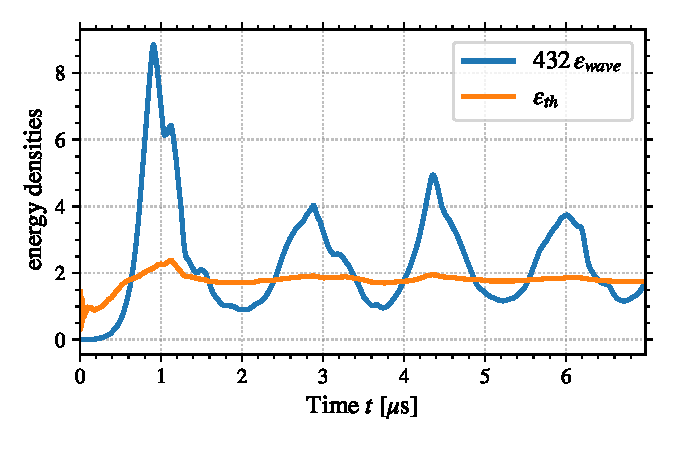
\includegraphics[width=\defaultwidth]{Ion_Trapping_criter_bis}
      \caption{Temporal evolution of the wave energy density (scaled) compared to the thermal energy density.}
      \label{fig-tempITcrit}
    \end{figure}
    
    In \cref{fig-tempITcrit}, as expected the period of the oscillations of $\epsilon_{\rm wave}$ is $T_{NL} = 1.5\,\micro\second$.
    But here, we can see that when the criteria \cref{eq-criteriaIT} is fulfilled, the temporal derivative of the wave energy density increases, which means that the wave growing rate is positive.
    However, some time after the moment in violated the criteria is violated ($\tau = 0.40 \pm 0.07 \,\micro\second$ on the four oscillations), the wave abruptly stop rising but decreases instead.
    This delay between the time the ions should be trapped and the time the wave stop growing in most certainly due to the ion inertia, as we have $\tau \sim T_B$.
    
    A complementary results is presented in \cref{subsec-VDFIAW} but solving the dispersion relations what we present in the next section.
    
      